\documentclass[11pt]{article}

\usepackage{hyperref}
\usepackage{listings}
%for dotex
\usepackage[pdftex]{graphicx}
\usepackage[pdf]{graphviz}
\usepackage[boxed]{algorithm2e} %end for dote
\usepackage{color}

% "define" Scala
\lstdefinelanguage{scala}{
  morekeywords={abstract,case,catch,class,def,%
    do,else,extends,false,final,finally,%
    for,if,implicit,import,match,mixin,%
    new,null,object,override,package,%
    private,protected,requires,return,sealed,%
    super,this,throw,trait,true,try,%
    type,val,var,while,with,yield},
  otherkeywords={=>,<-,<\%,<:,>:,\#,@},
  sensitive=true,
  morecomment=[l]{//},
  morecomment=[n]{/*}{*/},
  morestring=[b]",
  morestring=[b]',
  morestring=[b]"""
}

\lstset{ %
    language=scala,
    identifierstyle=\textbf
}

\title{Activity Trail Design}
\author{Maxim Noah Khailo}
\begin{document}
\maketitle
\section{Purpose}

We need to track all important activity of the system, both machine and human so that
our customers can keep track and organize their business.

\section{Forces}

Forces are problems we have to balance.

\begin{itemize}
    \item Activity is both human and machine.
    \item Machine activity can lead to human activity and vice versa.
    \item The information for each activity needs to be viewable. 
    \item You can view activities from multiple perspectives.
\end{itemize}


\section{Data Structure}

The following data structure design is motivated by the fact that we want to linearize 
events along many dimensions. It is composed of two parts, activities and doubly linked
lists along dimensions, where each dimension is a set of these linked lists where the head
is used to represent the start of the activity along that dimension. 


\newpage
\subsection{Activity}

An activity tracks changes to state made by both the computer and human actors.

We use the term Activity here instead of Event because events are a type of activity, and
activity implies a grouping.

\begin{lstlisting}
    case class Activity(
        id: Id, 
        type: String, 
        data: Json, 
        created: Instant)
\end{lstlisting}

One requirement is that the activity stores all data needed to visualize and compute on that activity. The type is used to understand how to decode the json for visualization.

An activity object is also immutable since it tracks changes to state but is NOT state.

\subsection{Connection}

Each activity exists in doubly-linked lists in multiple dimensions.

We connect activities together instead of linking them. Linking is traditionally used
as a term to mean pointer. Instead, we will store a two way \emph{Connection}

\begin{lstlisting}
    case class Connection(
        id: Id, 
        dimension: Id, 
        activity: Id, 
        previous: Id, 
        next: Id, 
        head: Id)
\end{lstlisting}

Each activity is connected by a two way connection creating a doubly linked list. Each
connection belongs to some dimension and in each dimension an activity belongs to only
one list. 

Each list has a head activity and the head activity has a connection where
the \emph{previous} points to the tail and the \emph{next} points to an activity next in time.

Each connection points to the head for optimization purposes. We can create an
index on the head to do quick queries based on dimension and head activity for that dimension.

\subsection{Dimensions}

So what are dimensions and how do they help model activities trails? Dimensions are essentially
a precomputed linearization of events based on a logical grouping.

\begin{lstlisting}
    case class Dimension(
        id: Id, 
        name: String, 
        description: String)
\end{lstlisting}

For example, we can look at activities for a customer. So we can have a \emph{customer\_activity}
dimension which will have a head activity that contains the customer.id in the json.

Another example, we may want to look at activities for an order. So we can have an \emph{order\_activity}
dimension which will have a head activity that contains the order.id in the json.

Another example, we may want to look at all activities by an admin. So we can have an \emph{admin\_activity}
dimension.

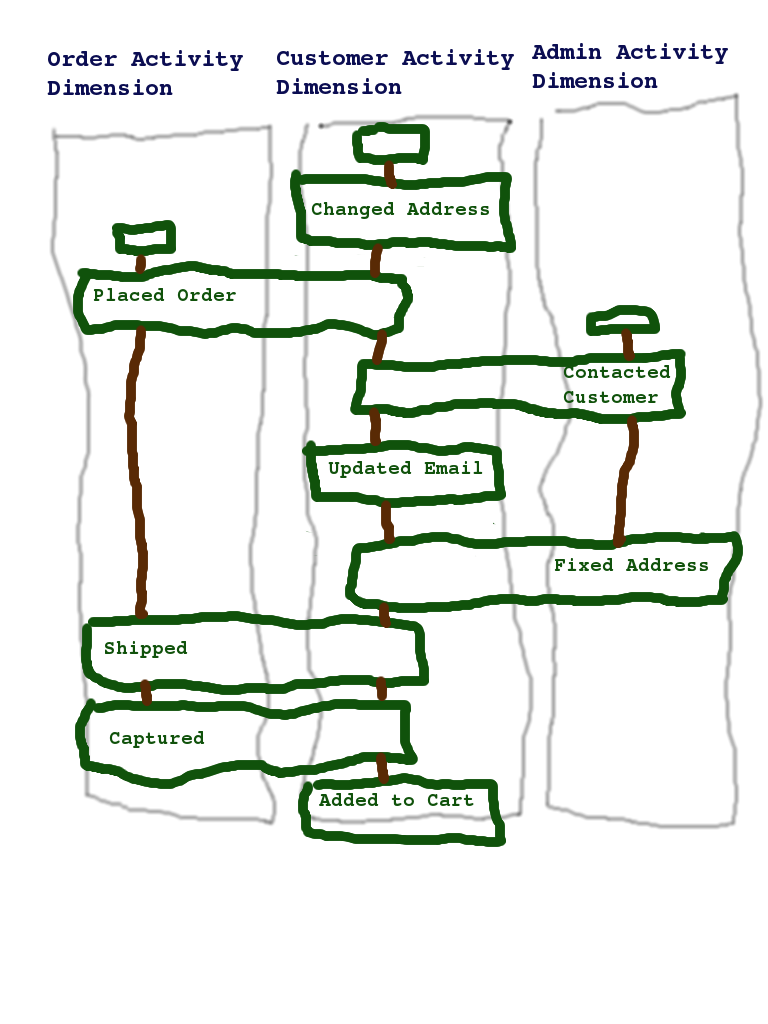
\includegraphics[scale=0.40]{dimension}

\section{Visualization}

One requirement for an activity is that all the data necessary for visualization is stored
in the JSON. While this will increase the amount of data stored, it will improve performance
in the UI by reducing the amount of queries. 

\section{Navigation}

One huge advantage to the data structure is that you can easily navigate it along multiple
dimensions efficiently. This provides interesting UI options in the future when you need
to jump from one view of activities to another.

\section{Pros}
\begin{enumerate}
    \item Performance. Cachable completely in Elastic Search
    \item Simplified UI. Activity trail can use the search api instead of hitting DB.
        We can use existing search infrastructure to filter activity trail.
    \item Simplified schema. DB schema is super simple and extensible as we add more dimensions.
        Otherwise we would have to store nulled ids in columns, or have different tables for
        different trails. 
    \item Sets us up for implementing workflows.
    \item Implementing watch and assignment is easy because of how dimensions work. You can
        watch an order, or a customer, or an admin, etc.
\end{enumerate}

\section{Cons}

There are many problems to this design.

\begin{enumerate}
    \item Adding an activity requires adding it to multiple
lists in many dimensions. 
    \item Size used is greater because each activity stores all data needed for visualization.
    \item Tracking activity is now explicit. Either phoenix needs changes or we create
           Kafka consumers which look at db changes and create the activity objects.
\end{enumerate}

\end{document}
